

\section{Method}
\begin{figure*}[t]
    \centering
    
\includegraphics[width=\linewidth]{sections/image/fig1.png}
    \caption{
        Overview of the LGDWT-GS framework.
        The model introduces frequency-domain regularization through global and local DWT losses.
        Combined supervision (L1, SSIM, and global DWT and local DWT) enhances structural stability and textural fidelity.
        Black and blue arrows represent operation and gradient flows, respectively.
    }
    \label{fig:method1}
\end{figure*}
We introduce the LGDWT-GS framework, which integrates frequency-domain supervision into the 3DGS  pipeline to improve few-shot 3D reconstruction.  
Then, we extend this framework to a multispectral version that jointly reconstructs RGB and NIR modalities under a shared 3D geometry.
% ===================== Subsection =====================
\subsection{LGDWT-GS Framework}

The proposed method extends the original 3DGS by introducing frequency-aware supervision through global and local (patch-wise) DWT losses. 
This integration enhances large-scale structural consistency and fine-grained texture recovery without modifying the differentiable splatting renderer. In few-shot settings, only a small number of sparse points can be reconstructed by COLMAP~\cite{schonberger2016sfm} due to limited view overlap. 
To obtain a denser and more stable initialization, depth priors and multi-view stereo reconstructions are used to generate additional pseudo-points, forming a more complete geometric basis for the Gaussian representation. 
Each Gaussian primitive is parameterized by a mean vector, covariance matrix, color, and opacity.

During training, the differentiable rasterizer projects these Gaussians into the image plane, and the rendered outputs are optimized against ground-truth views using a composite loss function,shown in Equation \ref{eq:ltotal}, that jointly balances spatial, perceptual, and frequency domain objectives

\begin{equation}
\mathcal{L}_{\text{total}} =
\mathcal{L}_{\text{L1}} +
\mathcal{L}_{\text{SSIM}} +
\alpha \mathcal{L}_{\text{gDWT}} +
\beta \mathcal{L}_{\text{pDWT}}.
\label{eq:ltotal}
\end{equation}

\noindent $\mathcal{L}_{\text{L1}}$ ensures pixel-wise fidelity, $\mathcal{L}_{\text{SSIM}}$ enforces structural similarity, $\mathcal{L}_{\text{gDWT}}$ and $\mathcal{L}_{\text{pDWT}}$ regularizes global and local frequency components, respectively. 
The weighting factors $\alpha$ and $\beta$ control the relative contribution of global and patch-wise DWT supervision during optimization. The overall proposed method with this loss function is shown in  Figure~\ref{fig:method1}.

\subsubsection{Global DWT Supervision}

The global DWT loss enforces large-scale frequency consistency between rendered and ground-truth images, promoting structural stability across views.  
Each image is decomposed using a one-level Haar wavelet transform into four frequency subbands. The LL subband represents the LF approximation of the image and preserves its coarse global structure. The LH subband captures horizontal HF components corresponding to vertical edges. The HL subband captures vertical HF components corresponding to horizontal edges. The HH subband contains diagonal HF information that highlights fine, corner-like details.


 $I_{LL}$ captures coarse structural information and global illumination, 
$I_{LH}$ and $I_{HL}$ represent horizontal and vertical edge responses, and $I_{HH}$ encodes fine textures and noise. Fig.~\ref{fig:wavelet_subbands}. The global DWT loss Equation \ref{eq:global_dwt} term is defined as follows:
% \begin{equation}
% \mathcal{L}_{\text{global-DWT}} =
% \sum_{s \in \{LL,LH,HL,HH\}}
% w_s \, \|\hat{I}_{s} - I_{s}\|_1,
% \label{eq:global_dwt}
% \end{equation}

\begin{equation}
\mathcal{L}_{\text{Global-DWT}} =
\sum_{s \in \{LL, LH, HL, HH\}}
w_s \, \|\widehat{\mathbf{I}}_{S} - \mathbf{I}_{S}\|_1,
\label{eq:global_dwt}
\end{equation}

where $w_s$ denotes the frequency weight for each subband.  
To mitigate overfitting to unstable HF regions ~\cite{yang2023freenerf}, the HH component is included but assigned a weight near zero ($w_{HH} \!\approx\! 0$).  
This formulation aligns global frequency structures between rendered and reference images, ensuring coherent reconstruction of both LF and mid-frequency content while suppressing noisy HF artifacts.

\begin{figure}[!t]
    \centering
    
    \subfloat[]{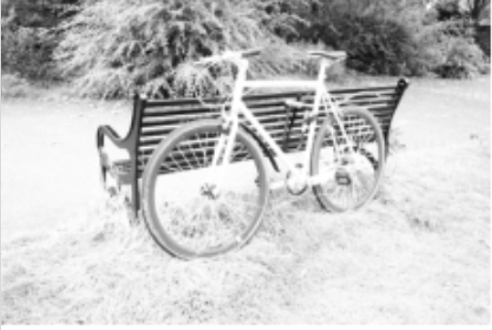
\includegraphics[width=0.22\linewidth]{sections/image/1.png}\label{fig_ll}}
    \hfil
    \subfloat[]{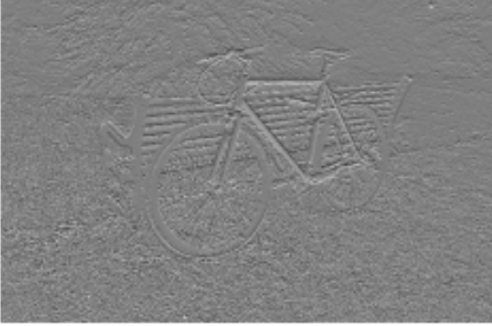
\includegraphics[width=0.22\linewidth]{sections/image/2.png}\label{fig_lh}}
    \hfil
    \subfloat[]{
\includegraphics[width=0.22\linewidth]{sections/image/3.png}\label{fig_hl}}
    \hfil
    \subfloat[]{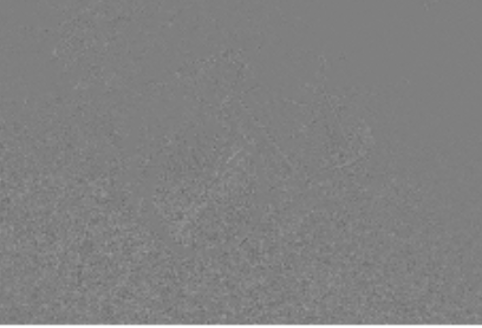
\includegraphics[width=0.22\linewidth]{sections/image/4.png}\label{fig_hh}}
    
    \caption{Wavelet decomposition of the input image into four subbands:  
    (a) LL (approximation),  
    (b) LH (horizontal),  
    (c) HL (vertical),  
    (d) HH (diagonal).}
    \label{fig:wavelet_subbands}
\end{figure}







\subsubsection{Patch-wise DWT Supervision}

Although global supervision enforces overall frequency consistency, local regions may still exhibit under-reconstruction, particularly where fine HF details are embedded within smooth, LF areas.  
To address this, patch-wise DWT supervision is introduced to refine these regions by locally emphasizing frequency balance. Rendered and ground-truth images are divided into non-overlapping patches of fixed size and stride.  
Each patch is independently analyzed to detect local frequency imbalance, guided by a Low-frequncy energy($E_{LF}$) metric that quantifies the dominance of LF versus HF content  Equation \ref{eq:energy}.  
Each image is first decomposed via a one-level Haar wavelet transform:
% \[
% I \xrightarrow{\text{DWT}} \{I_{LL}, I_{HF}\},
% \]
where $I_{LL}$ denotes the low frequency (structural) subband and $I_{HF}$ represents the aggregated high frequency components $(I_{LH}, I_{HL}, I_{HH})$.  
The $E_{LF}$ for each spatial location is defined as:
\begin{equation}
E_{LF}(x,y) =
\frac{\|\mathbf{I}_{LL}(x,y)\|_1}{
\|\mathbf{I}_{LL}(x,y)\|_1 + \|\mathbf{I}_{HF}(x,y)\|_1},
\label{eq:energy}
\end{equation}

Regions with low $E_{LF}$ values, defined as pixels whose $E_{LF}$ falls below a percentile based threshold that is treated as a hyperparameter and empirically set to the lowest 20\% of the $E_{LF}$ distribution per image, correspond to areas where structural information is weak or where HF details are missing in LF regions, as illustrated in Figure~\ref{fig:lfmap}.  
These regions are therefore prioritized for localized frequency refinement.

For each selected patch, one-level Haar wavelet transform is applied, and weighted losses are computed on the HF subbands to enhance local detail reconstruction. The patch-level loss Equation \ref{eq:patch_dwt} is defined as:
\begin{equation}
\mathcal{L}_{\text{Patch-DWT}} =
\frac{1}{N_p}\sum_{p=1}^{N_p}
\sum_{B \in \{LH, HL\}}
\|\widehat{\mathbf{I}}^{\,p}_{B} - \mathbf{I}^{\,p}_{B}\|_1,
\label{eq:patch_dwt}
\end{equation}

\noindent where $N_p$ denotes the number of selected patches and $b$ the corresponding frequency band.  
This localized supervision improves fine-grained reconstruction by reinforcing HF corrections within LF regions, sharpening object boundaries, and restoring texture details while maintaining global stability.

\begin{figure}[!t]
    \centering
    
    \subfloat[]{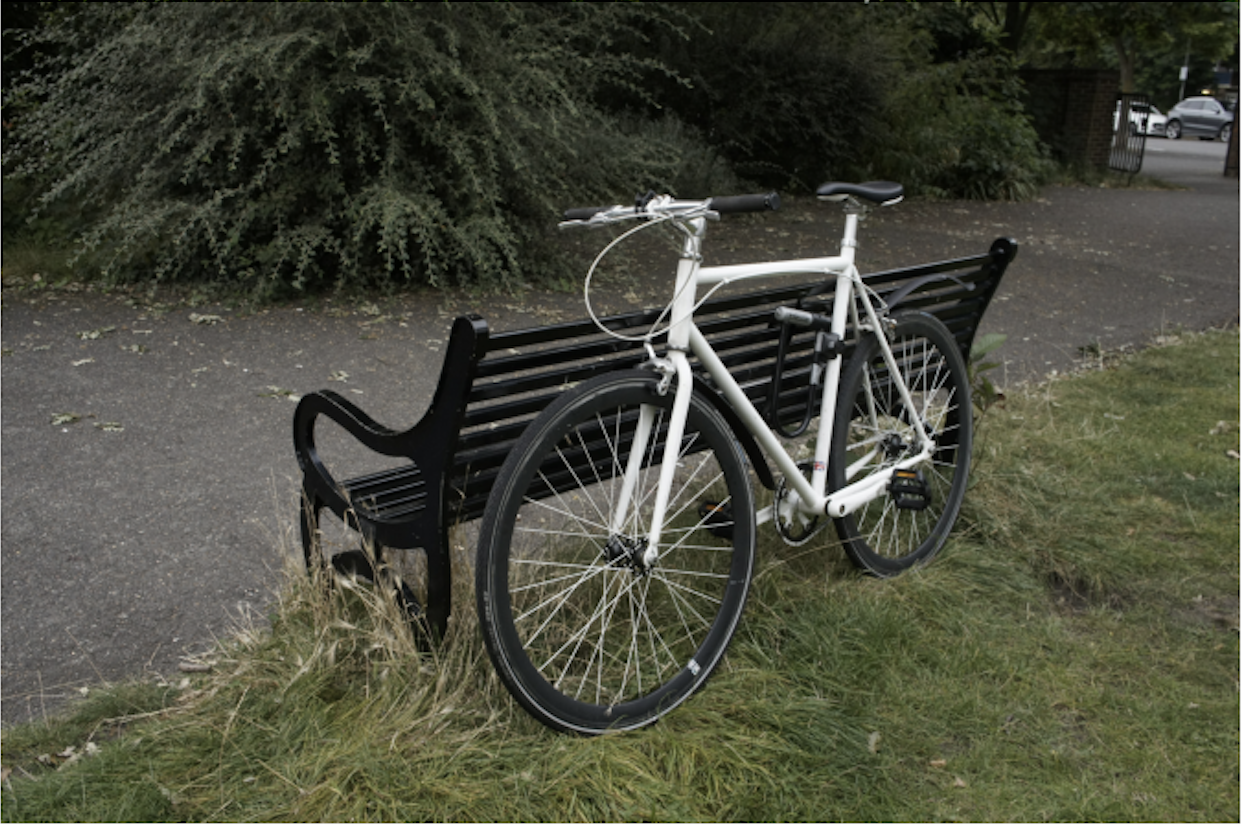
\includegraphics[width=0.48\linewidth]{sections/image/b1.png}\label{fig_lf_gt}}
    \hfill
    \subfloat[]{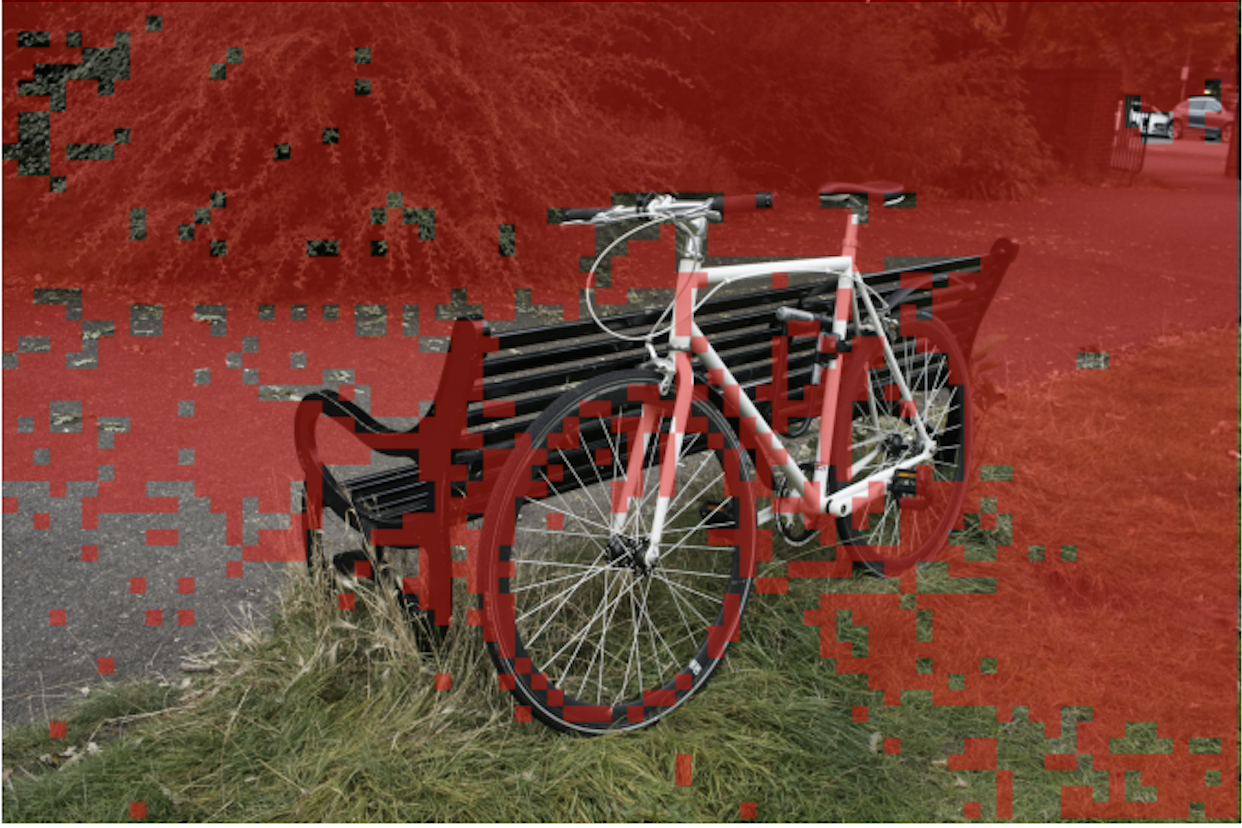
\includegraphics[width=0.48\linewidth]{sections/image/b2.png}\label{fig_lf_map}}

    \caption{
        $E_{LF}$ map used for patch selection:  
        (a) Ground Truth,  
        (b) $E_{LF}$ Map.  
        Red regions denote low $E_{LF}$ values, indicating weak LF stability or missing HF details and revealing spatial frequency imbalance in the reconstruction.
    }
    \label{fig:lfmap}
\end{figure}




% ===================== Subsection =====================
\subsection{MultiSpectral Extension}

The LGDWT-GS framework is extended to support dual-modality reconstruction, jointly modeling RGB and NIR images under a shared 3D geometry.  
This multispectral formulation introduces cross-spectral supervision, improving both geometric fidelity and spectral alignment across modalities. To initialize the geometry, pseudo-RGB images are first generated by combining the Red, Green, and Red-Edge spectral channels.  
These pseudo-RGB images are used as inputs to COLMAP to estimate camera poses and generate the initial sparse point cloud.  
The resulting structure provides reliable geometric alignment across all spectral bands, even in sparse-view conditions.

The RGB and NIR data are stored in separate but spatially aligned folders, sharing identical intrinsic and extrinsic camera parameters.  
This setup ensures pixel-level correspondence between modalities and enables synchronized multispectral loading during training.  
Optional depth priors can also be incorporated to further densify the initialization and stabilize reconstruction in regions with limited multiview overlap. Each Gaussian primitive maintains shared geometric parameters while encoding modality-specific color attributes.
Two-pass differentiable rasterization is then applied to produce the corresponding renderings.
% \[
% \hat{I}_{RGB},\, \hat{I}_{NIR} =
% \text{Render}_{RGB}(G),\;
% \text{Render}_{NIR}(G),
% \]
allowing both branches to be optimized jointly under a unified geometry while preserving spectral distinctions.

Supervision combines reconstruction objectives from both the RGB channel and the NIR channel Equation \ref{eq:multi}:
\begin{equation}
\mathcal{L}_{\text{Multi}} =
\mathcal{L}_{\text{RGB}} + \lambda_{\text{NIR}}\, \mathcal{L}_{\text{NIR}},
\label{eq:multi}
\end{equation}


\noindent where it $\lambda_{NIR}$ controls the relative contribution of the NIR branch.  
During densification, new Gaussians are spawned in regions exhibiting high residuals in either spectral channels Equation \ref{eq:mask}:
\begin{equation}
\text{mask} = \max(\text{RGB}_{\text{res}}, \text{NIR}_{\text{res}}),
\label{eq:mask}
\end{equation}

\noindent ensuring that both spectral domains selectively guide geometric refinement. This shared-geometry, dual-appearance design promotes cross-spectral coherence and enhances fine-detail reconstruction under sparse-view conditions.

\begin{figure}[t]
    \centering
    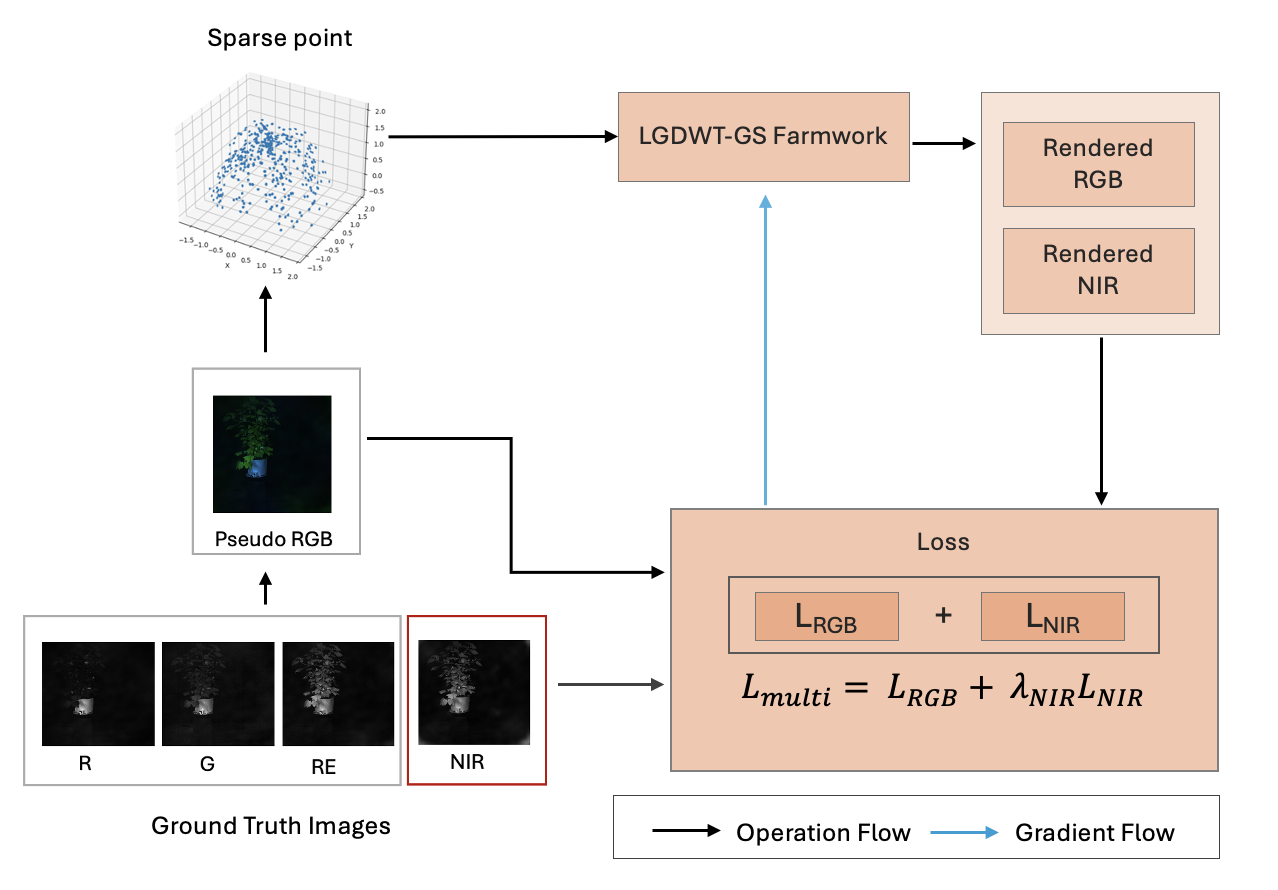
\includegraphics[width=\linewidth]{sections/image/multi.png}
    \caption{
        Multispectral LGDWT-3DGS framework. 
        Pseudo-RGB images (constructed from Red, Green, and Red-Edge bands) are used for COLMAP-based pose estimation and sparse reconstruction. 
        RGB and NIR chanells are then jointly optimized under a shared geometry using cross-spectral supervision and DWT-based frequency regularization, improving geometric consistency and spectral alignment under sparse-view scenarios.
    }
    \label{fig:method2}
\end{figure}



\subsection{Dataset}
% \label{sec:dataset}

To construct the proposed multispectral greenhouse dataset, we employed the MSIS-AGRI-1-A system: a snapshot multispectral camera equipped with four spectral bands centered at 580~nm (Green), 660~nm (Red), 735~nm (Red Edge), and 820~nm (NIR) Figure~\ref{fig:multispectral_samples}.  
The camera uses a global shutter CMOS sensor with 4~MP resolution and integrates Anti-X-Talk\texttrademark~technology to minimize spectral leakage between channels, ensuring radiometrically accurate and high-contrast measurements.  
Each capture was synchronized with a four-channel LED illumination module operating at the same wavelengths to maintain consistent spectral lighting across all bands.  
Before data collection, both cameras were calibrated for intrinsic and extrinsic parameters using a checkerboard target to ensure precise geometric alignment.

Each scene corresponds to an individual plant species sorghum, tomato, alocasia, cotton, and grape captured inside a controlled greenhouse imaging station Figure~\ref{fig:env_setup}.  
The setup includes a motorized turntable, a uniform black background, and a multispectral LED illumination system designed to ensure radiometric consistency and suppress ambient reflections.  
Two identical cameras were placed on opposite sides of the turntable, providing dual viewpoints.  
For each fixed horizontal position, the cameras were vertically translated across four discrete heights to capture multiple canopy layers.  
Each plant was imaged at ten rotational steps (36° increments) using the motorized turntable, with two reference cube markers attached for rotation tracking and geometric calibration.  
Each acquisition session generated approximately 80–100 multispectral frames per scene, yielding almost 500 spatially aligned spectral images across all plant species.

\begin{figure*}[!t]
    \centering
    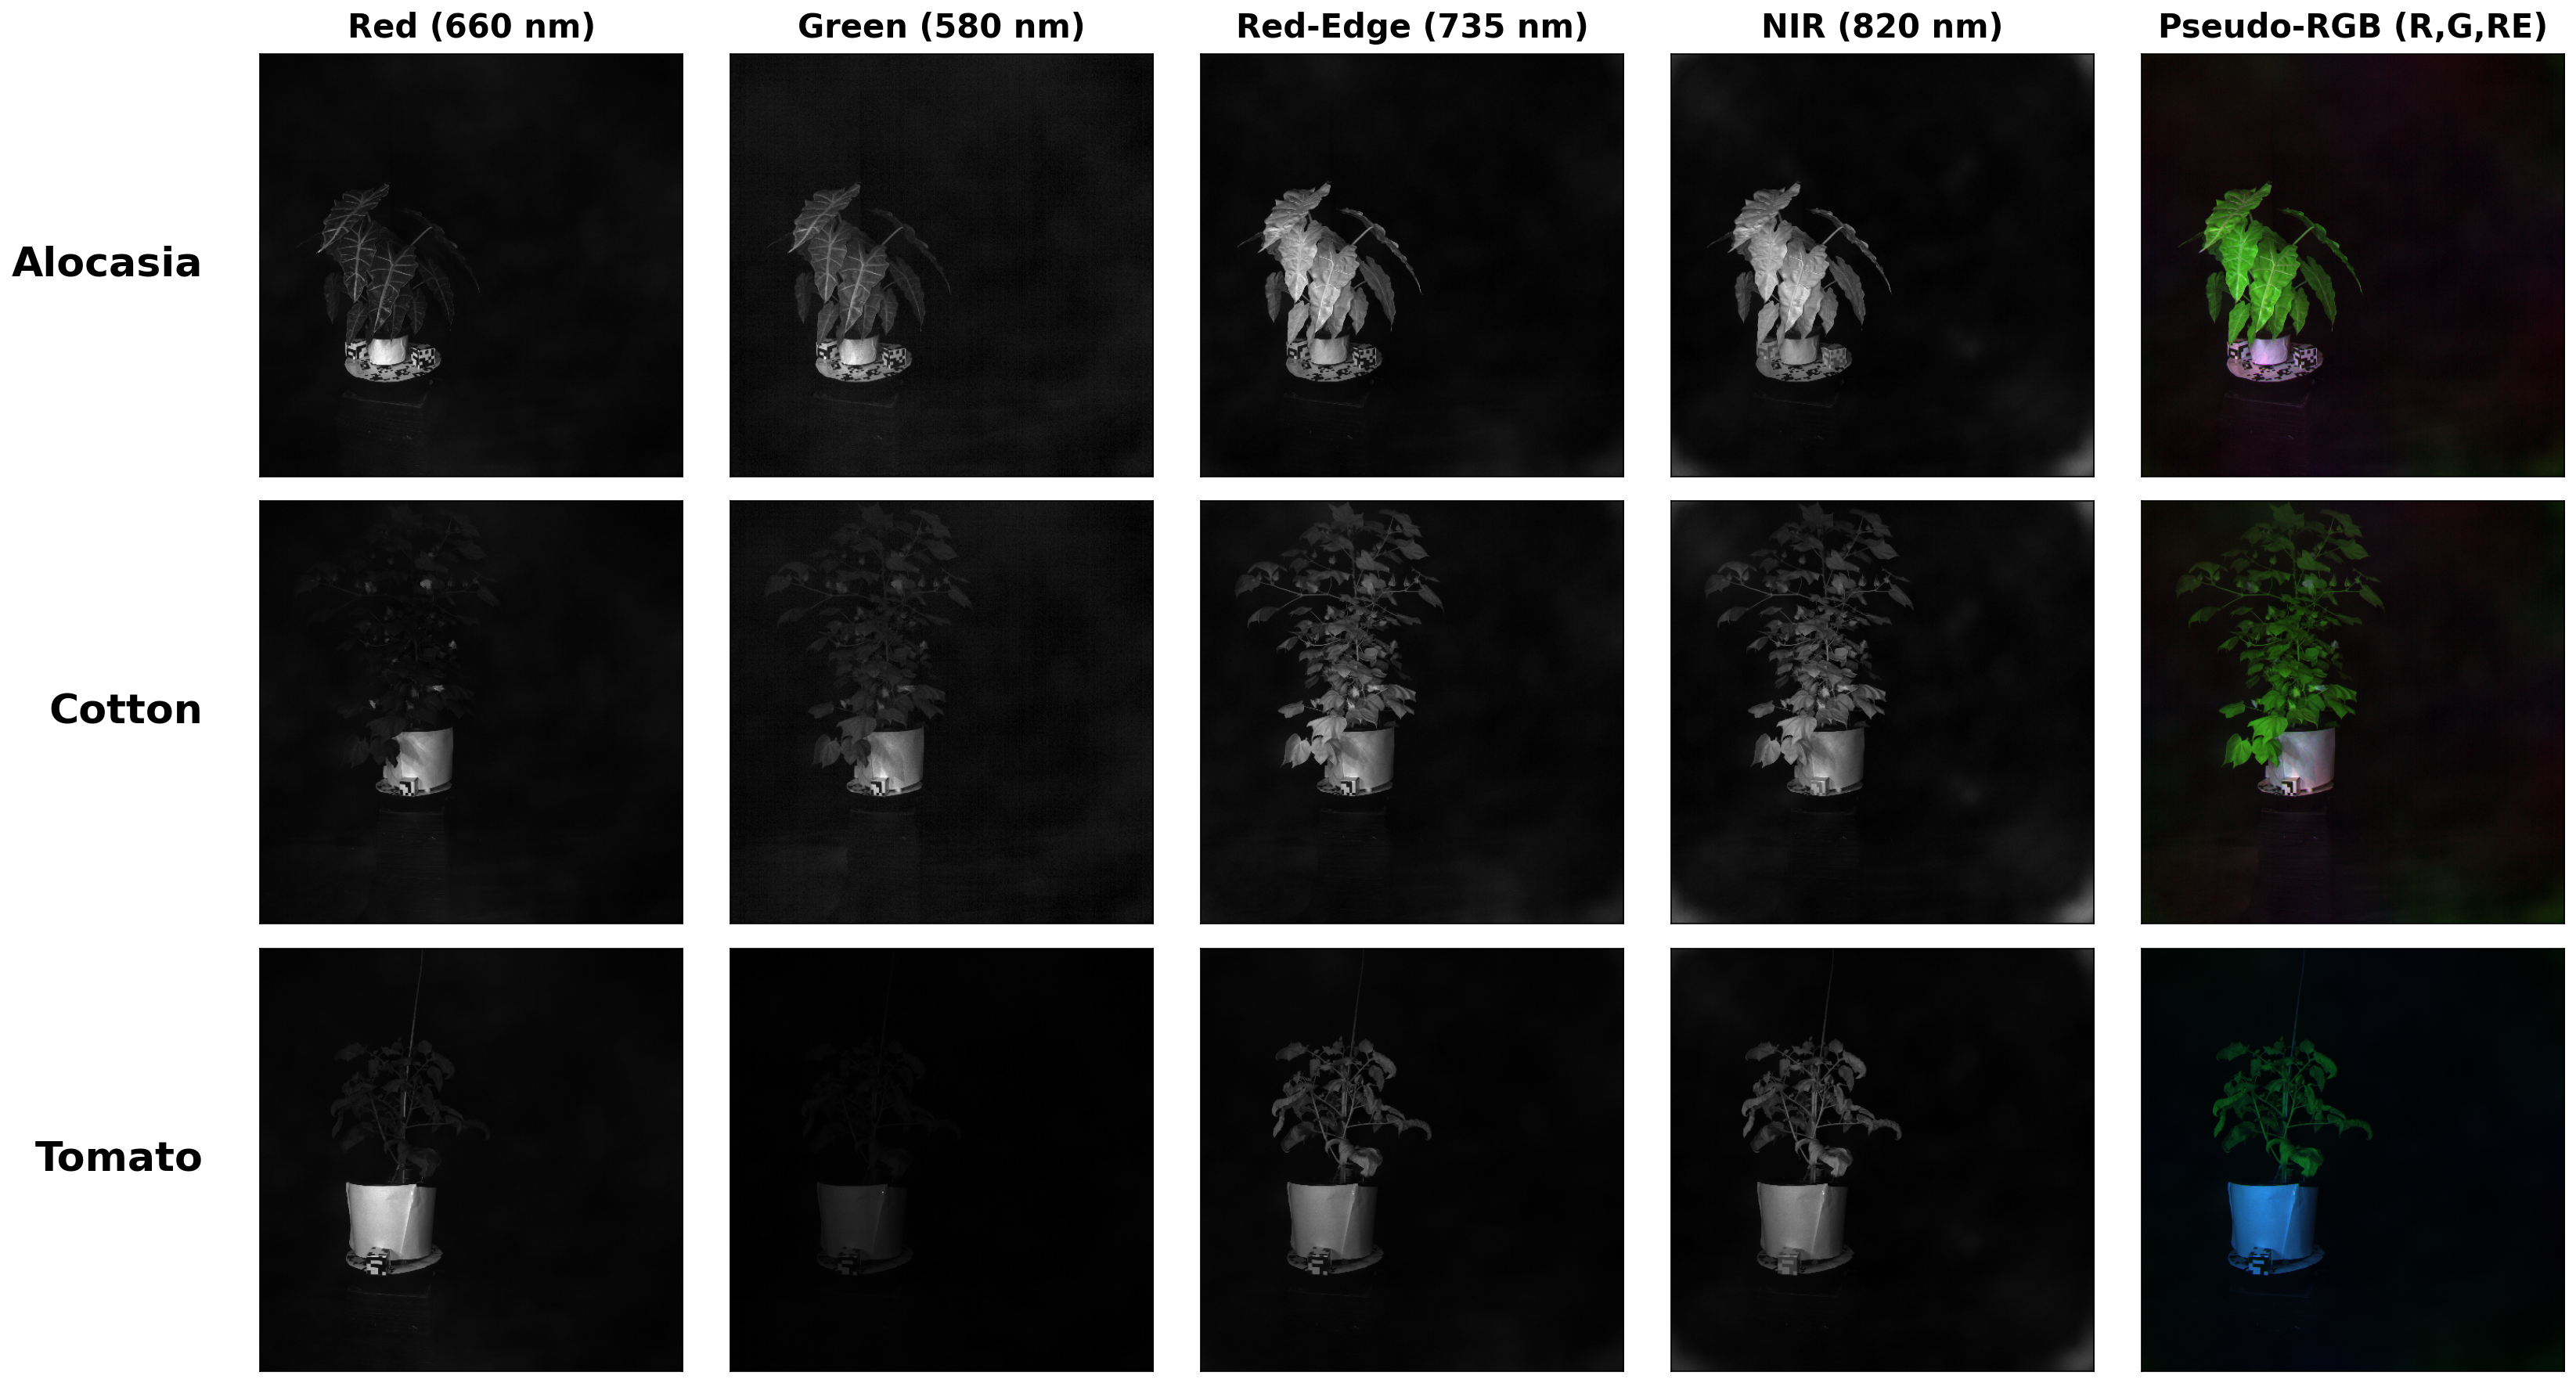
\includegraphics[width=0.95\textwidth]{sections/image/spectral_grid_3plants.png}
    \caption{Example spectral channels for three representative plant scenes. Columns correspond to 580~nm (Green), 660~nm (Red), 735~nm (Red Edge), and 820~nm (NIR) bands. The final column shows the pseudo-RGB composite used for COLMAP reconstruction.}
    \label{fig:multispectral_samples}
\end{figure*}

\begin{figure}[!t]
    \centering
    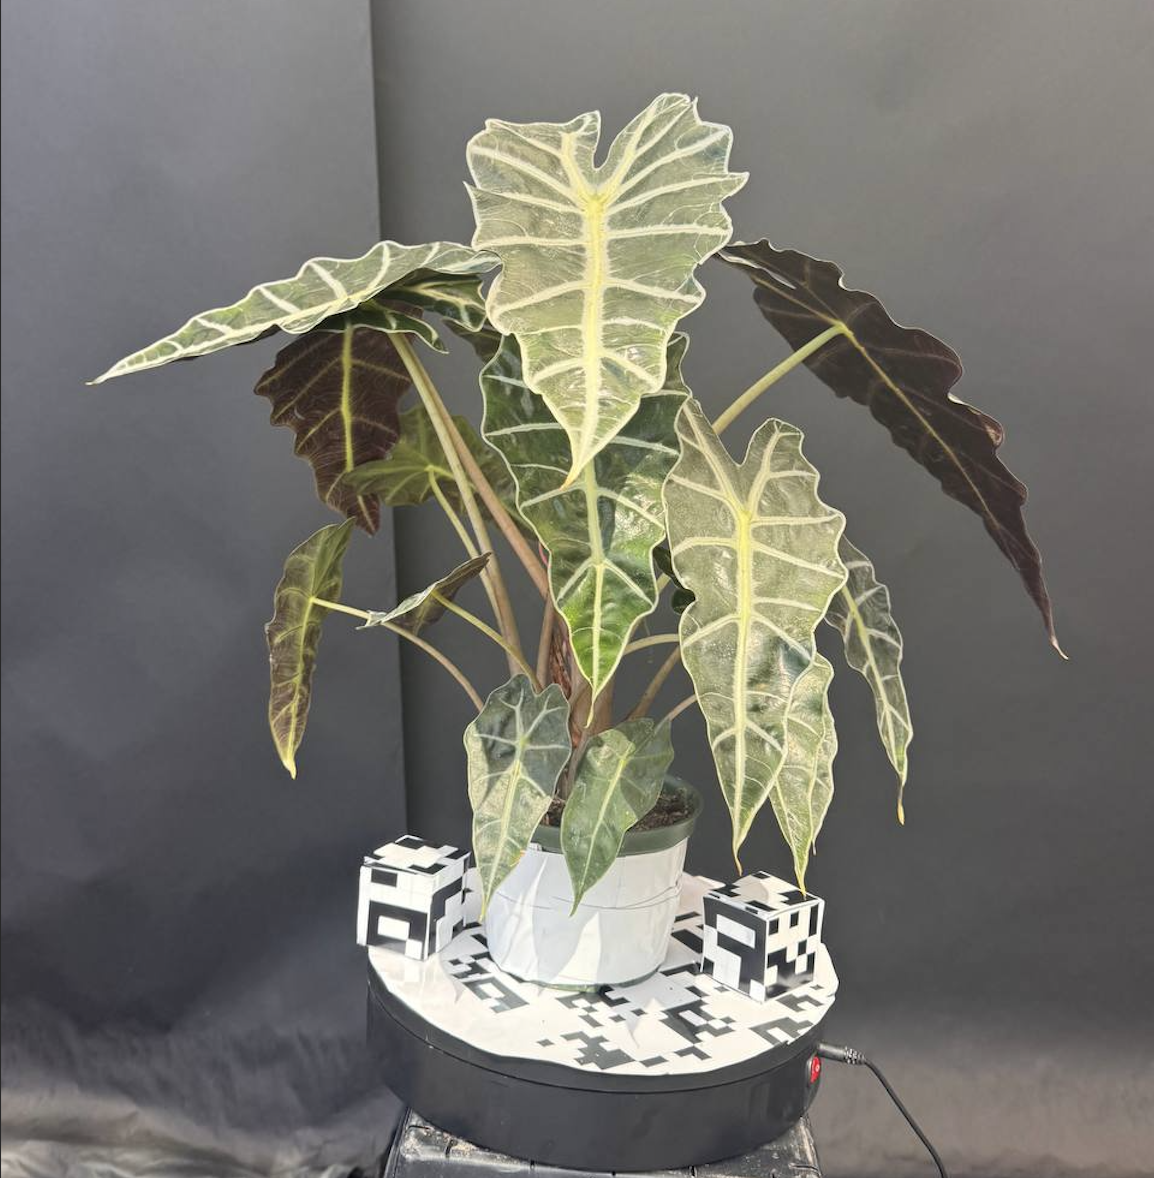
\includegraphics[width=0.75\linewidth]{sections/image/setup.png}
    \caption{Greenhouse imaging setup. The MSIS-AGRI-1-A camera, LED illumination system, motorized turntable, and cube reference markers used for geometric calibration are shown.}
    \label{fig:env_setup}
\end{figure}


For each acquisition, four spectral bands were recorded simultaneously, forming a co-registered multispectral image cube $\{I_{R}, I_{G}, I_{RE}, I_{NIR}\}$.  
A pseudo-RGB composite was generated from the Red, Green, and Red Edge channels to facilitate Structure-from-Motion (SfM) reconstruction using COLMAP.  
Reconstructed camera poses, sparse point clouds, and scene bounds were used as geometric initialization for multispectral 3DGS training.  
This preprocessing ensures spatial alignment between spectral modalities and enables consistent cross-spectral supervision during reconstruction.